\chapter{Class Weapons} \label{Weapons}

\subsection{Introduction to Class Weapons}

Class weapons are weapons of great power that can only be wielded by certain classes. Each weapon has a back story of where it came from and how it received it's powers. The weapons, will provide enhanced abilities for anyone that is successful in wielding them. The weapons all have consciousnesses imbued within them and must accept the wielder as worthy in order for the potential of the weapon to be unleashed. 

\begin{commentbox}{Determining the class to persue}
	To determine which class weapon can be found, you can simply roll a d8 to determine where the story will tend.
	\hline
	\begin{multicols}{4}
		\begin{description}
			\item[1:] Rogue 
			\item[2:] Warlock
			\item[3:] Druid
			\item[4:] Barbarian
			\item[5:] Paladin
			\item[6:] Reaper
			\item[7:] Cleric
			\item[8:] Re-roll
		\end{description}
	\end{multicols}
\end{commentbox}

\section{Class Weapons}

\section{Rogue Class Weapons}

\subsubsection{The Kingslayers}

The Kingslayers are legend to be twin daggers that have been used in the assassination of multiple kings throughout ancient times.The blades are said to have been crafted by the legendary Hassassin (a rogue assassin trained from birth to be the perfect killing machine). The blades are believed to be infused with dark and poisonous magic that can corrupt anything they pierce. The blades are made from a rare metal that was mined from a meteorite. The blades are believed to have been traded down in generations within a small cult of specially trained Hassassins. The cult was focused on removing kings and nobles of high status if they did not fit their agendas. The blade is rumored to have vanished after the line of the Hassassins vanished during a world war when the planet divided its governments and broke into strife.

\begin{center}
	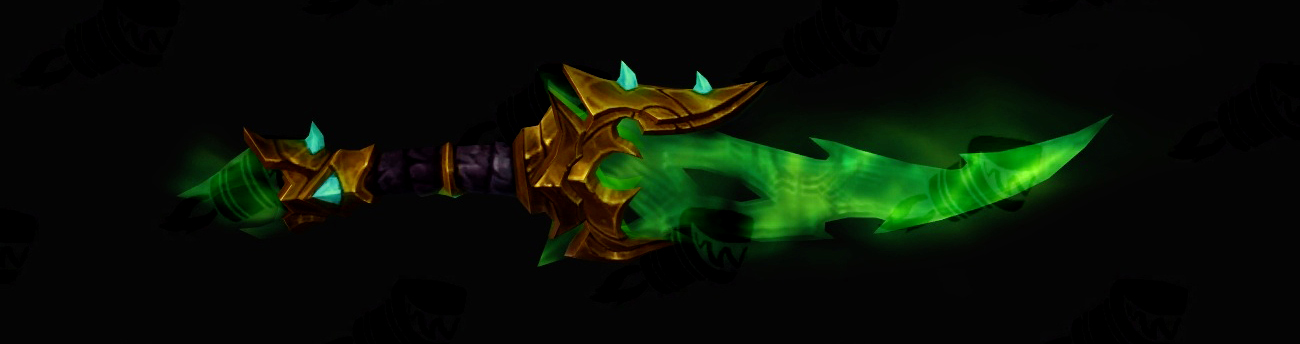
\includegraphics[width=\linewidth]{img/weapons/kingslayer-green.jpg}
	
	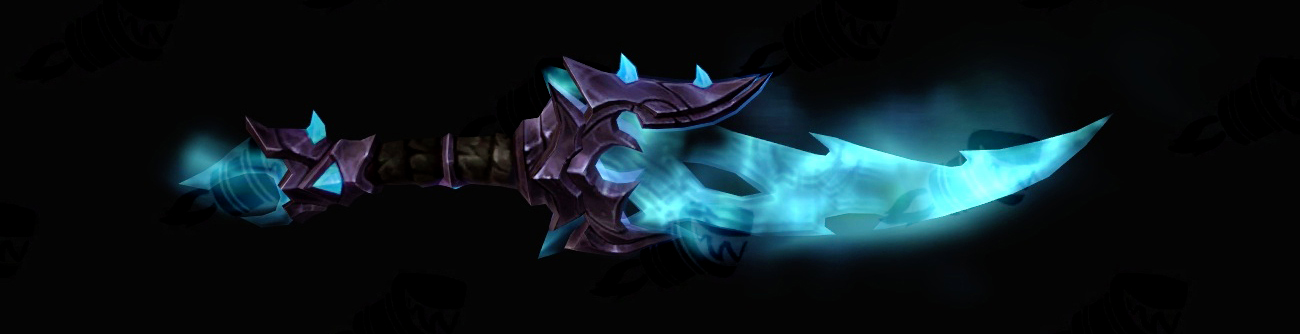
\includegraphics[width=\linewidth]{img/weapons/kingslayer-blue.jpg}
\end{center}

\subsubsection{Potential}

The Kingslayers want to remain hidden or be wielded by a member of the Hassassin bloodline. The Blades can sense the bloodline of their wielder and reject anyone not of the Hassassin descent. There are two blades and each have similar properties but different damage types.

\begin{commentbox}{Kingslayers\footnote{Weapon (daggers), artifact (requires attunement by a rogue)}}
	You gain a +3 bonus to attack and damage rolls made with this magic weapon. When you hit an enemy with the green blade you will deal 1d6 necrotic damage and 1d6 poison damage. When you hit an enemy with the blue blade you will deal 1d6 cold damage and 1d6 lightning damage. The damage will change to d10's if the target is not aware of the Rogues presence.
	
	The target of two successive attacks with both blades must make a constitution saving throw. On a fail, they take 5d6 poison damage. The DC for this save is the wielders level + their constitution.
	
	While a rogue wields The Kingslayers in combat it will look like the rogue has a shadowy presence. The wielder of the Kingslayers gains a +2 to stealth while wielding them.
	
	If a rogue of an non-Hassassin bloodline tries to attune to The Kingslayers they have to make a d20 roll. At a 18 or below The Kingslayers will reject you and deal 3d10 Poison damage and 2d10 Necrotic damage. At a 19 or 20 you over power the will of the weapon and make it yours.
	
	Proficiency with a daggers allows you to add your proficiency bonus to the attack roll for any attack you make with them.
	
	If the wielder of the Kingslayers dies, the Kingslayers will sink into the killer and attempt to kill it (unless it is within the Hassassin bloodline).
\end{commentbox}

\subsubsection{Finding The Kingslayers}

Within the Pluvian Realm, there exists an area referred to as crystal lake. This area is almost a perfect circle cut into the middle of the Pluvian wilderness. The region is a large flat lake that is iced over with multiple feet of thick ice. In the very center is a large fossilized pirate ship covered in ice. The wind is strong over this area and the air very cold. Surrounding the lake is forest. At the bottom of the ice in the depths of the river are solid crystals of various kinds. This gives the appearance of a shimmering surface when the sunlight is intense enough in this area.

The ship in the ice is frozen over with thick layers of ice. On the side of the ship is the name ``Charlotte'', which is the name of the ship. The ship and surrounding lake was frozen due to an Ice dragon that resides in a nearby cave. The ship contained the last Hassassin to wield the Kingslayers as well as the blades themselves. The Hassassin was not killed when the ship was frozen but rather preserved in the ice of the vessel. The Hassassin and the daggers are frozen within the hull of the ship alongside the Hassassin. If the vessel is thawed, it will come alive as will the frozen Hassassin. To obtain the Kingslayers one must kill the Hassassin.

\begin{center}	
	
\includegraphics[width=0.485\linewidth]{img/terrain/winter-frozen-lake-reflection-blue-ice-green-trees-wallpaper-quotes.jpg}
	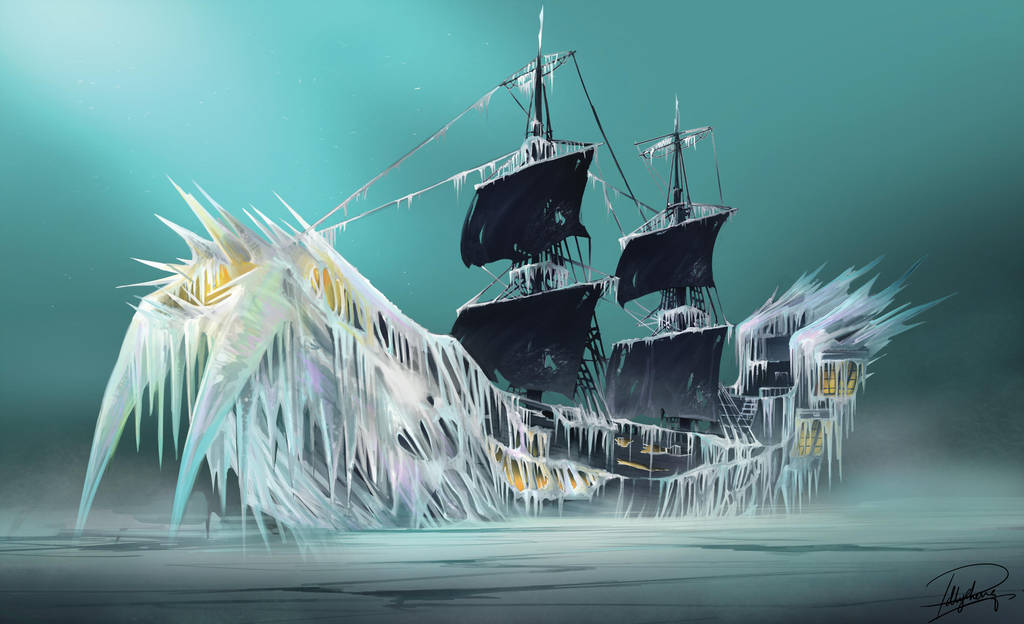
\includegraphics[width=0.50\linewidth]{img/ice_pirate_ship_by_pollychong_da47p92-fullview.jpg}
	
	\dndline
		
	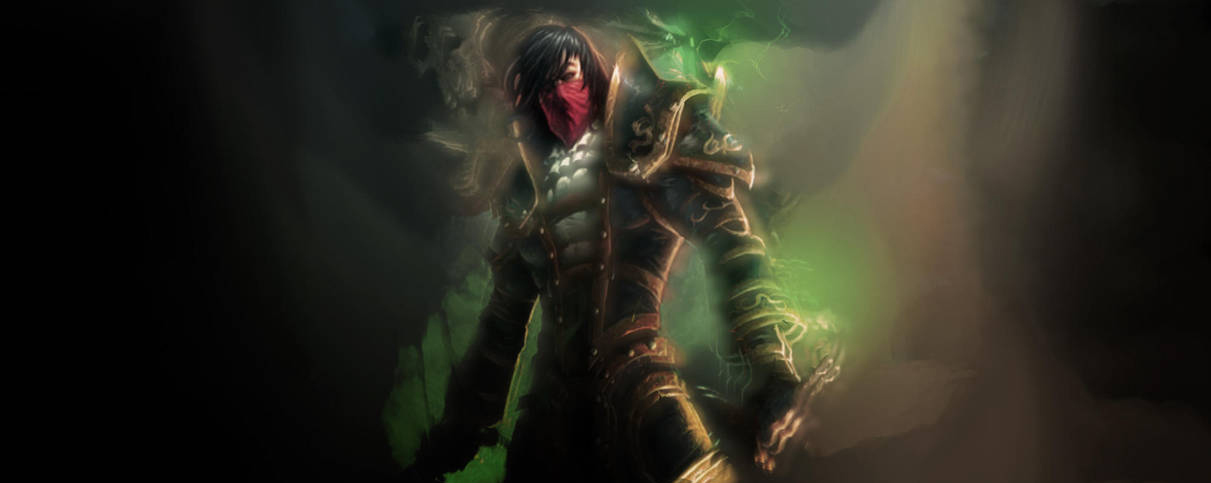
\includegraphics[width=\linewidth]{img/WoW/edwinvancleef.jpg}
\end{center}

\begin{monsterbox}{Weakened Hassassin}
	This character design is based on https://www.dndbeyond.com/monsters/assassin
	\begin{hangingpar}
		\textit{Medium humanoid, neutral evil}
	\end{hangingpar}
	\dndline%
	\basics[%
	armorclass = 16,
	hitpoints  = 98,
	speed      = 30 ft
	]
	\dndline%
	\stats[
	STR = \stat{11}, % This stat command will autocomplete the modifier for you
	DEX = \stat{18},
	CON = \stat{16},
	INT = \stat{13},
	WIS = \stat{11},
	CHA = \stat{10}
	]
	\dndline%
	\details[%
	% If you want to use commas in these sections, enclose the
	% description in braces.
	% I'm so sorry.
	languages = {Hassassin, Thieves' cant, Common},
	challenge = 10
	]
	\dndline%
	saving throws = DEX +7, INT +4
	
	skills = Acrobatics +6, Deception +3, Perception +3, Stealth +12
	
	damage resistance = Poison
	
	Senses = Passive Perception 13
	
	\dndline%
	\begin{monsteraction}[Assassinate]
		During its first turn or while vanished, the assassin has advantage on attack rolls against any creature that hasn't taken a turn. Any hit the assassin scores against a surprised creature is a critical hit.
	\end{monsteraction}	
	\begin{monsteraction}[Evasion]
		 If the assassin is subjected to an effect that allows it to make a Dexterity saving throw to take only half damage, the assassin instead takes no damage if it succeeds on the saving throw, and only half damage if it fails.		
	\end{monsteraction}	
	\begin{monsteraction}[Multiattack]
		The Hassassin makes two attacks.
	\end{monsteraction}
	\monstersection{Actions}
	\begin{monsteraction}[Kingslayer Attack]
		Melee Weapon Attack: +6 to hit, reach 5 ft., one target. Hit: See Kingslayer damage, replace the DC save effect with the following: the target must make a DC 15 Constitution saving throw, taking 24 (7d6) poison damage on a failed save, or half as much damage on a successful one.
	\end{monsteraction}
	\begin{monsteraction}[Light Crossbow]
		Ranged Weapon Attack: +6 to hit, range 80/320 ft., one target. Hit: 7 (1d8 + 3) piercing damage, and the target must make a DC 15 Constitution saving throw, taking 24 (7d6) poison damage on a failed save, or half as much damage on a successful one.
	\end{monsteraction}
	\monstersection{Legendary Actions}
	You can make 3 legendary actions per day. These are done after an action is done on any turn.
	\begin{monsteraction}[Vanish]
		You can magically wreath the area in smoke, vanishing from visibility. You remain concealed until performing an attack or successfully being perceived by another.
	\end{monsteraction}
\end{monsterbox}



\section{Warlock Class Weapons}

\subsubsection{Spine of the Condemned}

\subsubsection{Potential}

\subsubsection{Finding the Spine of the Condemned}

\section{Druid Class Weapons}

\subsubsection{Staff of Elune}


\begin{center}
	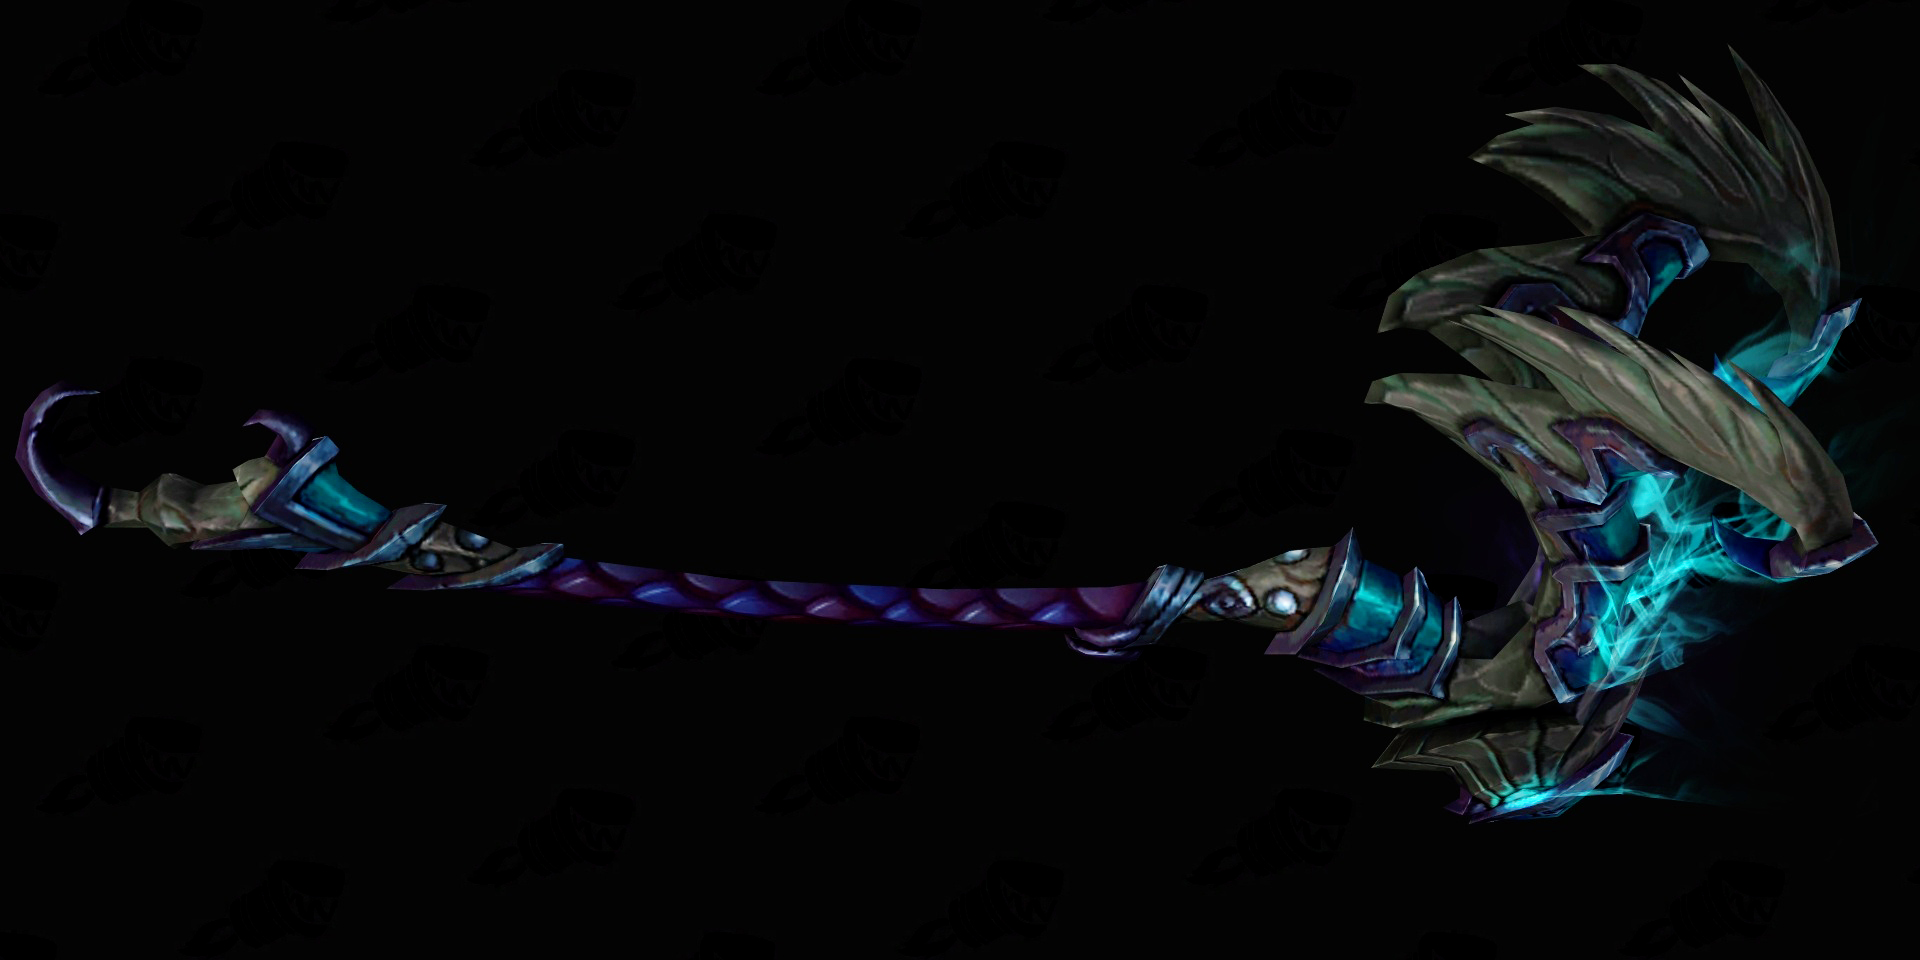
\includegraphics[width=\linewidth]{img/weapons/554329.jpg}
\end{center}

\subsubsection{Potential}



\subsubsection{Finding the Staff of Elune}

\section{Barbarian Class Weapons}

\subsubsection{Strom'kar the Warbreaker}

\subsubsection{Potential}

\section{Paladin Class Weapons}

\subsubsection{Ashbringer}

It is said that the righteousness of a man is determined by his ability to resist temptations and instead seek what is good for others. Legend has it that true righteousness has only ever been known by one man. An ancient king of Dalaran named Uther. They called him the light-bringer for his righteous acts. Uther reigned from a young boy after his father was killed in battle. He spent his life focused on maintaining peace from attacks from alternate realms and dimensions. It is believed that he was so charismatic that under his reign there was a one rule government. At the end of his life, he was blessed with the opportunity to ascend to a higher plane of existence due to his righteous acts. Upon doing so, he imbued his weapon, Ashbringer, with all of his physical abilities as he shed his body of his soul. It is said that he did this in the catacombs of Ironforge, the great capitol city that they ruled from in these times. The City is said to have been destroyed following the days of his reign when the world broke out into an age changing war. After centuries, all but remains of Ashbringer is but a legend.

\begin{center}
	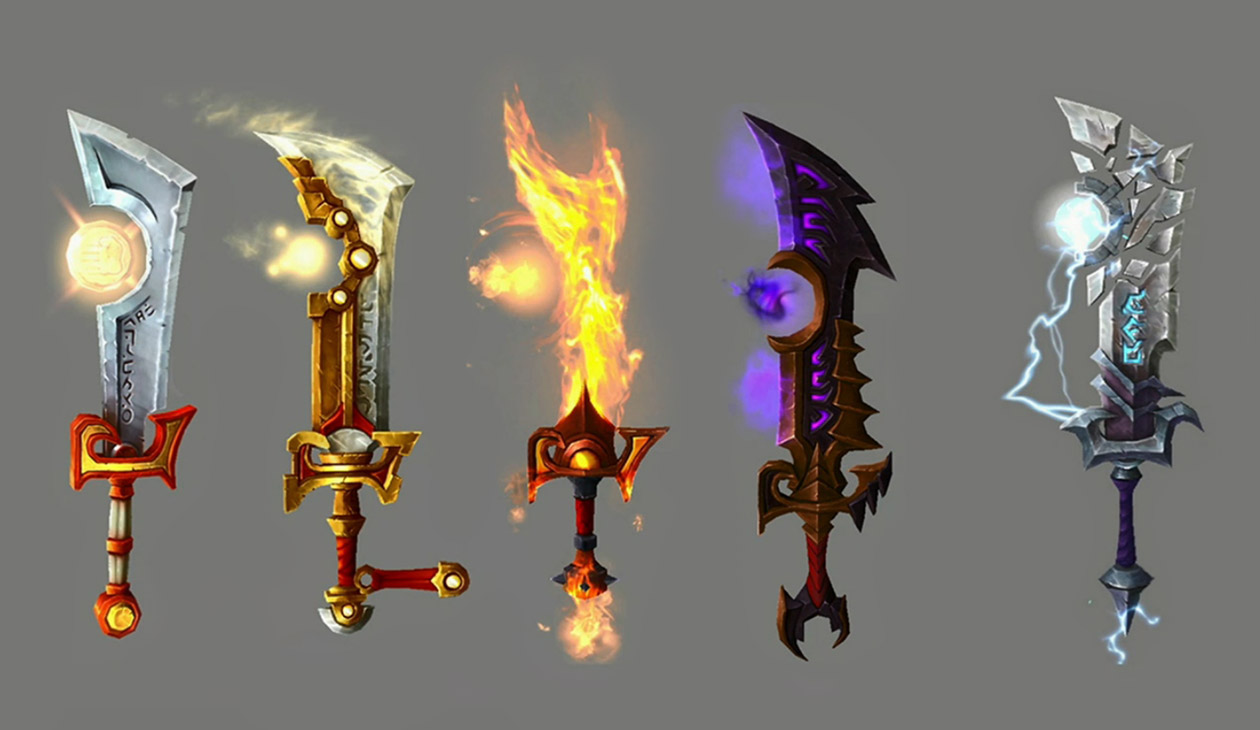
\includegraphics[width=\linewidth]{img/weapons/wowl-ashbringer.jpg}
\end{center}

\subsubsection{Potential}

The Ashbringer weapon wants to be wielded by a righteous character. 

\begin{commentbox}{Ashbringer\footnote{Some information taken from https://www.dndbeyond.com/magic-items/351998-the-ashbringer}\footnote{Weapon (greatsword), artifact (requires attunement by a paladin)}}{\tiny }
	
	
	You gain a +3 bonus to attack and damage rolls made with this magic weapon. When you hit an enemy you will deal 1d6 fire damage and 1d6 radiant damage. The damage will change to d10's if the target is a fiend or an undead.
	
	While a Paladin wields The Ashbringer in combat it will look like the Paladin is burning with a holy flame. Any fiend or undead that attacks the wielder will take 1d6 fire damage and 1d6 radiant damage. When the wielder rolls a 20 against a fiends or an undead the wielder must a d100 roll. If the roll is less than half the wielders lvl then the fiend or undead will burn in holy flame and turn to ash immediately.
	
	If a Paladin of an evil alignment tries to attune to The Ashbringer they have to make a d20 roll. At a 18 or below The Ashbringer will reject you and deal 3d10 fire damage and 2d10 radiant damage. At a 19 or 20 you over power the will of the weapon and make it yours.
	
	With a successful roll to overcome the will of The Ashbringer while having an evil alignment will make The Ashbringers appearance will start to dull and become darker until it becomes fully corrupt. It will regain its former glory when its attuned to a paladin of a non evil alignment.
	
	Proficiency with a greatsword allows you to add your proficiency bonus to the attack roll for any attack you make with it.
	
	If the wielder of Ashbringer dies (by failing three death saves) then the life essence of the blade can leave the weapon and resurrect the player to full. The weapon after this point becomes useless.
\end{commentbox}

\subsubsection{Finding Ashbringer}

Ashbringer is located in an underground vault within the city of Ironforge. Ironforge is located within the Pluvian Forest and has been hidden with time. Ironforge can only be spotted when winter. The snow covering the entrance is slightly melted from the super-heated thermal activities under the cities. The city is mainly collapsed but can be traversed if found. The main gate to the city is closed, but from an avalanche of rocks, part of it is accessible on one side. The Pluvian Forest contains a section stuck in time during an eternal winter, within this winter is where Ironforge is located. From the outside (space-view) this region appears normal, however upon a creature entering this large region, they are transported into a past time when it is winter. 

\begin{center}
	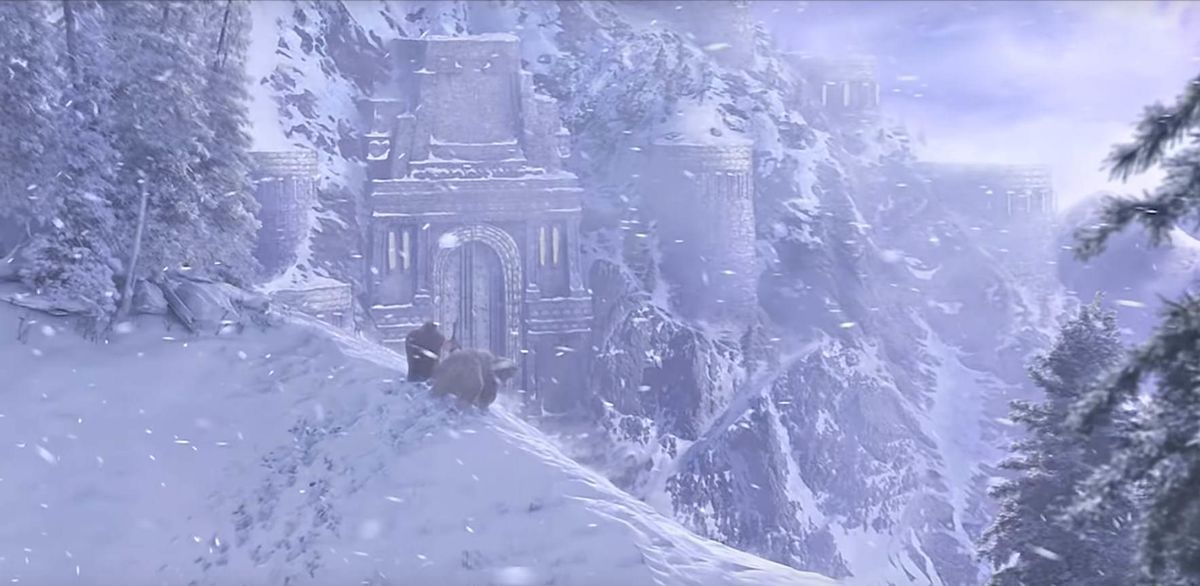
\includegraphics[width=\linewidth]{img/WoW/1200px-Ironforge_-_Classic_cinematic.jpg}
\end{center}

When entering Ironforge, the air is warm and a significant amount of steam is present rising from the thermal ducts throughout the city. The ducts in this state are full of lava that have broken through the lower gates of the vents. Within the center of the city is the kings chamber, where passage to the lower vaults is. Ashbringer is located in the depths of the vault. The vault is a series of large/high paths overlooking magma and lava pits that bubble and steam continually. The area is extremely warm. When approaching Ashbringer, the party will encounter the Firelord Ragnaros. Ragnaros will stop fighting if someone can successfully wield The Ashbringer weapon but will otherwise attack the party and chase them out of the vault.

\begin{center}
	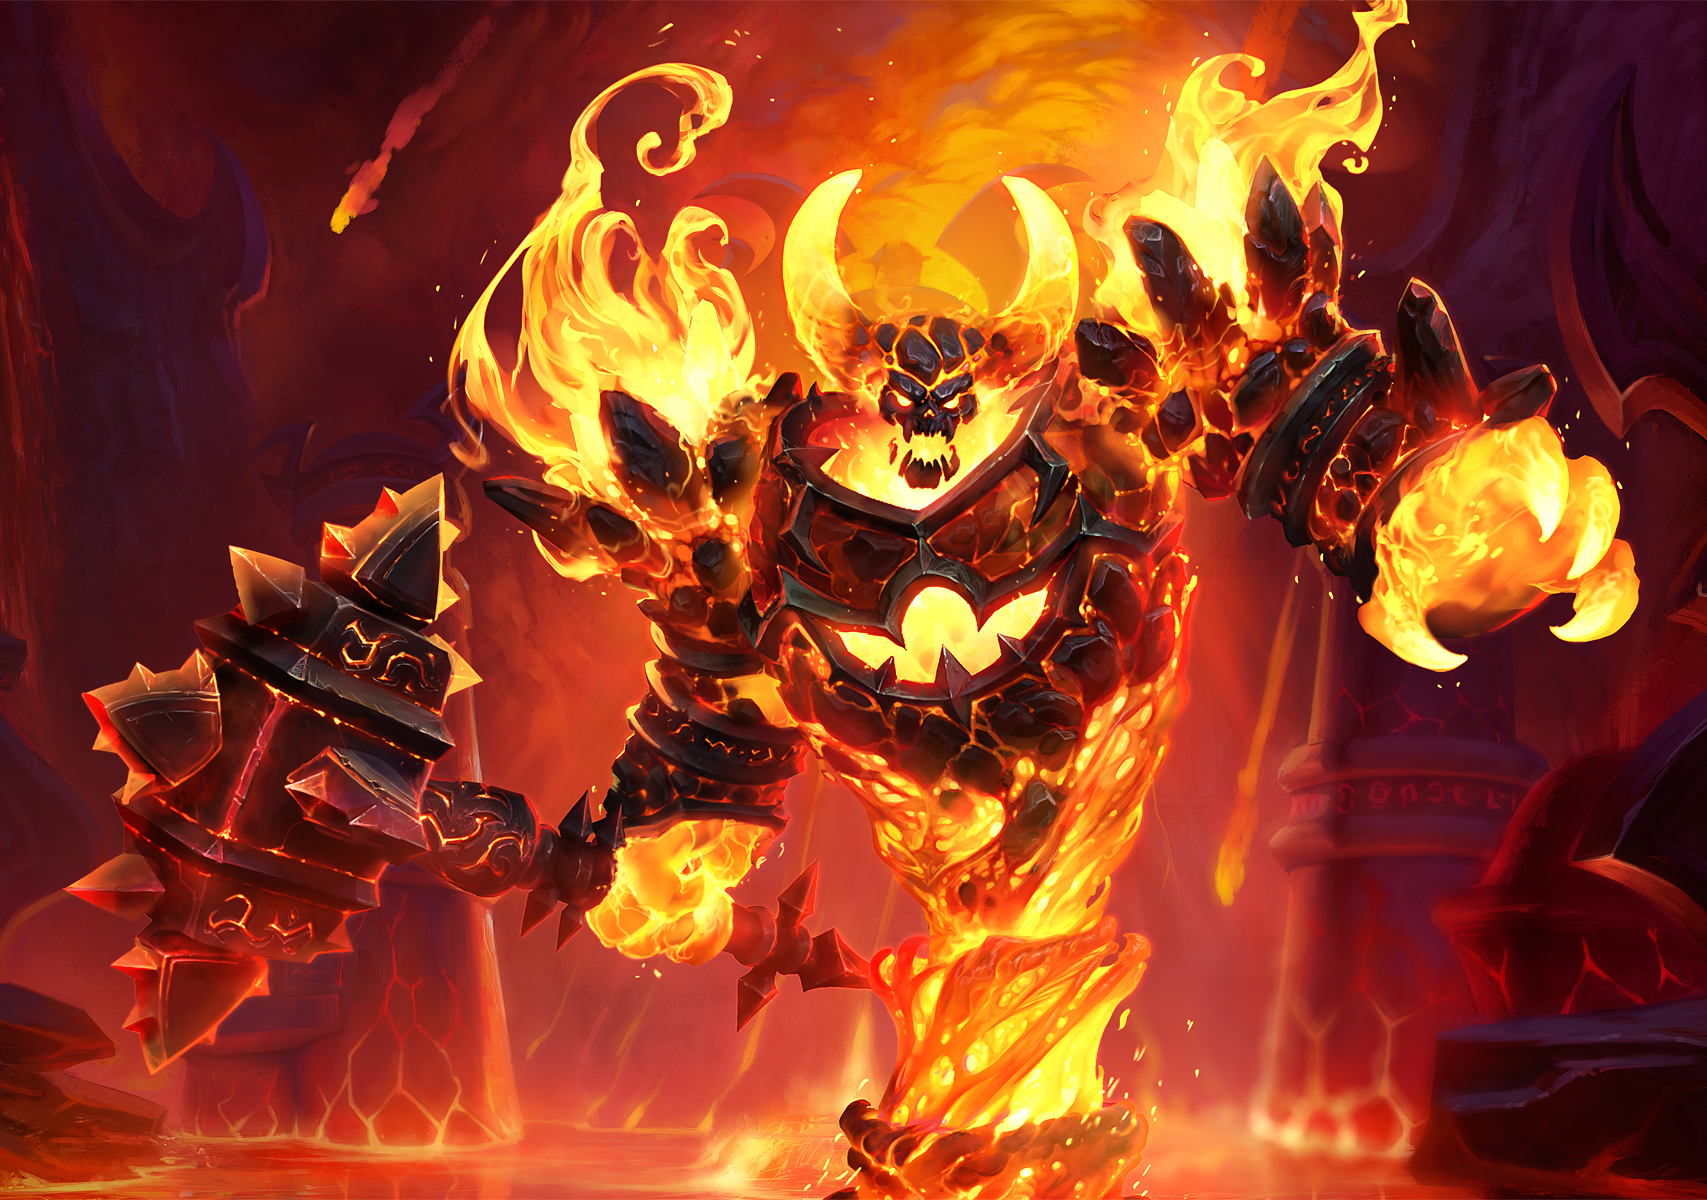
\includegraphics[width=0.515\linewidth]{img/WoW/ragnaros-1920x1200-heroes-of-the-storm-5781.jpg} 	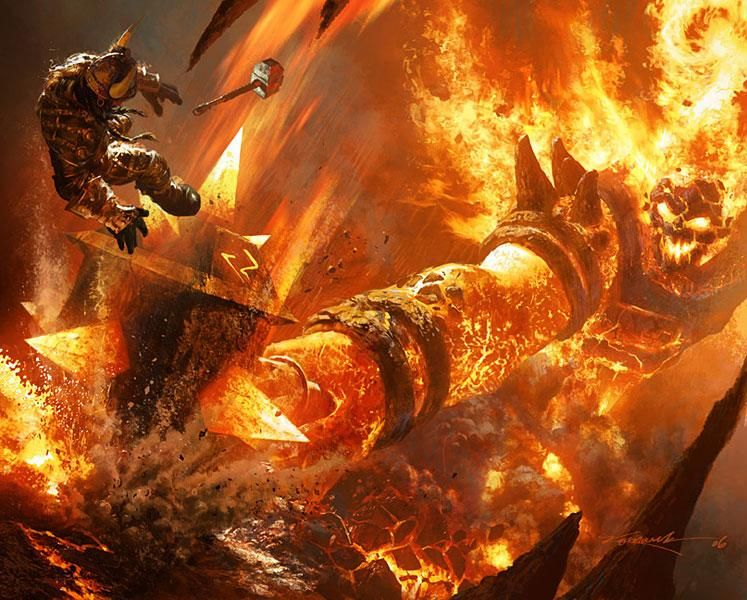
\includegraphics[width=0.45\linewidth]{img/WoW/b9e0808495e9cf3dcbbecedf3e4d5e32.jpg}
\end{center}

\begin{monsterbox}{Ragnaros The Firelord}
	This character design is taken from https://www.dndbeyond.com/monsters/82907-ragnaros
	\begin{hangingpar}
		\textit{Gargantuan Fiend, neutral evil}
	\end{hangingpar}
	\dndline%
	\basics[%
	armorclass = 23,
	hitpoints  = 533,
	speed      = 50 ft
	]
	\dndline%
	\stats[
	STR = \stat{30}, % This stat command will autocomplete the modifier for you
	DEX = \stat{20},
	CON = \stat{30},
	INT = \stat{30},
	WIS = \stat{24},
	CHA = \stat{30}
	]
	\dndline%
	\details[%
	% If you want to use commas in these sections, enclose the
	% description in braces.
	% I'm so sorry.
	languages = {All, Telepathy 5 miles},
	challenge = 30
	]
	\dndline%
	saving throws = STR +19, DEX +14, CON +19, INT +19, WIS +16, CHA +19
		
	skills = Deception +28, Insight +25, Perception +16, Persuasion +28
		
	damage resistance = Cold
	 
	damage immunities = Fire, Lightning, Poison; Bludgeoning, Piercing, and Slashing from Nonmagical Attacks that aren't Silvered
		
	condition immunities = Exhaustion, Petrified, Poisoned	
	
	Senses = Truesight 120 ft., Passive Perception 20
	
	\dndline%
	\begin{monsteraction}[Fear aura]
		Any creature hostile to Ragnaros that starts its turn within 20 feet of Ragnaros must make a DC 24 Wisdom saving throw, unless Ragnaros is incapacitated. On a failed save, the creature is frightened until the start of its next turn. If a creature's saving throw is successful, the creature is immune to Ragnaros's Fear Aura for the next 24 hours.
	\end{monsteraction}	
	\begin{monsteraction}[Death Throes]
		When Ragnaros dies, it explodes, and each creature within 30 feet of it must make a DC 20 Dexterity saving throw, taking 105 (30d6) fire damage on a failed save, or half as much damage on a successful one. The explosion ignites flammable objects in that area that aren't being worn or carried, and it destroys the balor's weapons.
	\end{monsteraction}	
	\begin{monsteraction}[Fire Aura]
		At the start of each of Ragnaros's turns, each creature within 5 feet of it takes 10 (3d6) fire damage, and flammable objects in the aura that aren't being worn or carried ignite. A creature that touches Ragnaros or hits it with a melee attack while within 5 feet of it takes 10 (3d6) fire damage.
	\end{monsteraction}	
	\begin{monsteraction}[Magic Weapon]
		The pit fiend's weapon attacks are magical.
	\end{monsteraction}	
	\begin{monsteraction}[Innate Spellcasting]
		The pit fiend's spellcasting ability is Charisma (spell save DC 23). Ragnaros can innately cast the following spells, requiring no material components:
		
		\begin{itemize}
			\item At will: detect magic, fireball, burning hands, charm person
		
			\item 3/day each: hold monster, wall of fire, 
		
			\item 2/day each: incendiary cloud, delayed blast fireball, dominate person
		
			\item 1/day each: meteor swarm, storm of vengeance 
		\end{itemize}
	\end{monsteraction}	
	\monstersection{Actions}
	\begin{monsteraction}[Multiattack]
		Ragnaros makes five attacks: one with its bite, two with its claw, one with its mace, and one with its lightning whip.
	\end{monsteraction}	
	\begin{monsteraction}[Bite]
		Melee Weapon Attack: +14 to hit, reach 5 ft., one target. Hit: 22 (4d6 + 8) piercing damage plus 14 (4d6) fire damage.  The target must succeed on a DC 21 Constitution saving throw or become poisoned. While poisoned in this way, the target can't regain hit points, and it takes 21 (6d6) poison damage at the start of each of its turns. The poisoned target can repeat the saving throw at the end of each of its turns, ending the effect on itself on a success.
	\end{monsteraction}	
	\begin{monsteraction}[Claw]
		Melee Weapon Attack: +19 to hit, reach 10 ft., one target. Hit: 19 (2d8 + 10) slashing damage.
	\end{monsteraction}	
	\begin{monsteraction}[Mace]
		Melee Weapon Attack: +19 to hit, reach 10 ft., one target. Hit: 17 (2d6 + 10) bludgeoning damage plus 35 (10d6) fire damage.
	\end{monsteraction}	
	\begin{monsteraction}[Lightning Whip]
		Melee Weapon Attack: +19 to hit, reach 30 ft., one target. Hit: 17 (2d6 + 10) slashing damage plus 35 (10d6) lightning damage, and the target must succeed on a DC 20 Strength saving throw or be pulled up to 25 feet toward Ragnaros
	\end{monsteraction}	
	\begin{monsteraction}[Polymorph]
		Ragnaros can take the form of a gargantuan molten titan (his actual form) or of any devil or demon and uses the stats of that form, if he is killed in one of these forms he begins regenerating in his lair and cant take form for a time, he is only killed if he dies in his actual form
	\end{monsteraction}	
	\begin{monsteraction}[Teleport]
		Ragnaros magically teleports, along with any equipment he is wearing or carrying, up to 120 feet to an unoccupied space it can see.
	\end{monsteraction}	
	\monstersection{Legendary Actions}
	Ragnaros can take 3 legendary actions, choosing from the options below. Only one legendary action option can be used at a time and only at the end of another creature's turn. Ragnaros regains spent legendary actions at the start of its turn.
	\begin{monsteraction}[Detect]
		Ragnaros makes a Wisdom (Perception) check.
	\end{monsteraction}
	\begin{monsteraction}[Lightning Whip]
		Ragnaros makes a Lightning whip attack.
	\end{monsteraction}
	\begin{monsteraction}[Use Spell (costs 2 actions]
		Ragnaros Casts one of his spells. expending a spell slot as normal
	\end{monsteraction}
	\monstersection{Description/Information}
	Ragnaros is actually a demon and devil fused into 1 being and is incredibly powerful, rivalling Asmodeus himself. When he wishes he can take the form of a gargantuan mountain of molten rock and fire or he can take the form of any demon or devil, There is a place on the material plane known as the Elemental Valley known for it containing portals to all 4 of the elemental planes, deep under this valley is where Ragnaros is locked for eternity,
\end{monsterbox}



\section{Grim Reaper Class Weapons}

\subsubsection{Scythe of the Unmaker}

The Scythe of the Unmaker is an ancient Scythe of legend. It is said that this weapon was wielded by the first Grim Reaper to exist. It is claimed that this Reaper stole the scythe from a god, Argus the Unmaker. The scythe is said to contain all of the souls of those slain by it. This is  where the power of the scythe is from. The wielder of the scythe is said to forever be cursed with the burdens of the souls it contains and will slowly be corrupted by its power.

\begin{center}
	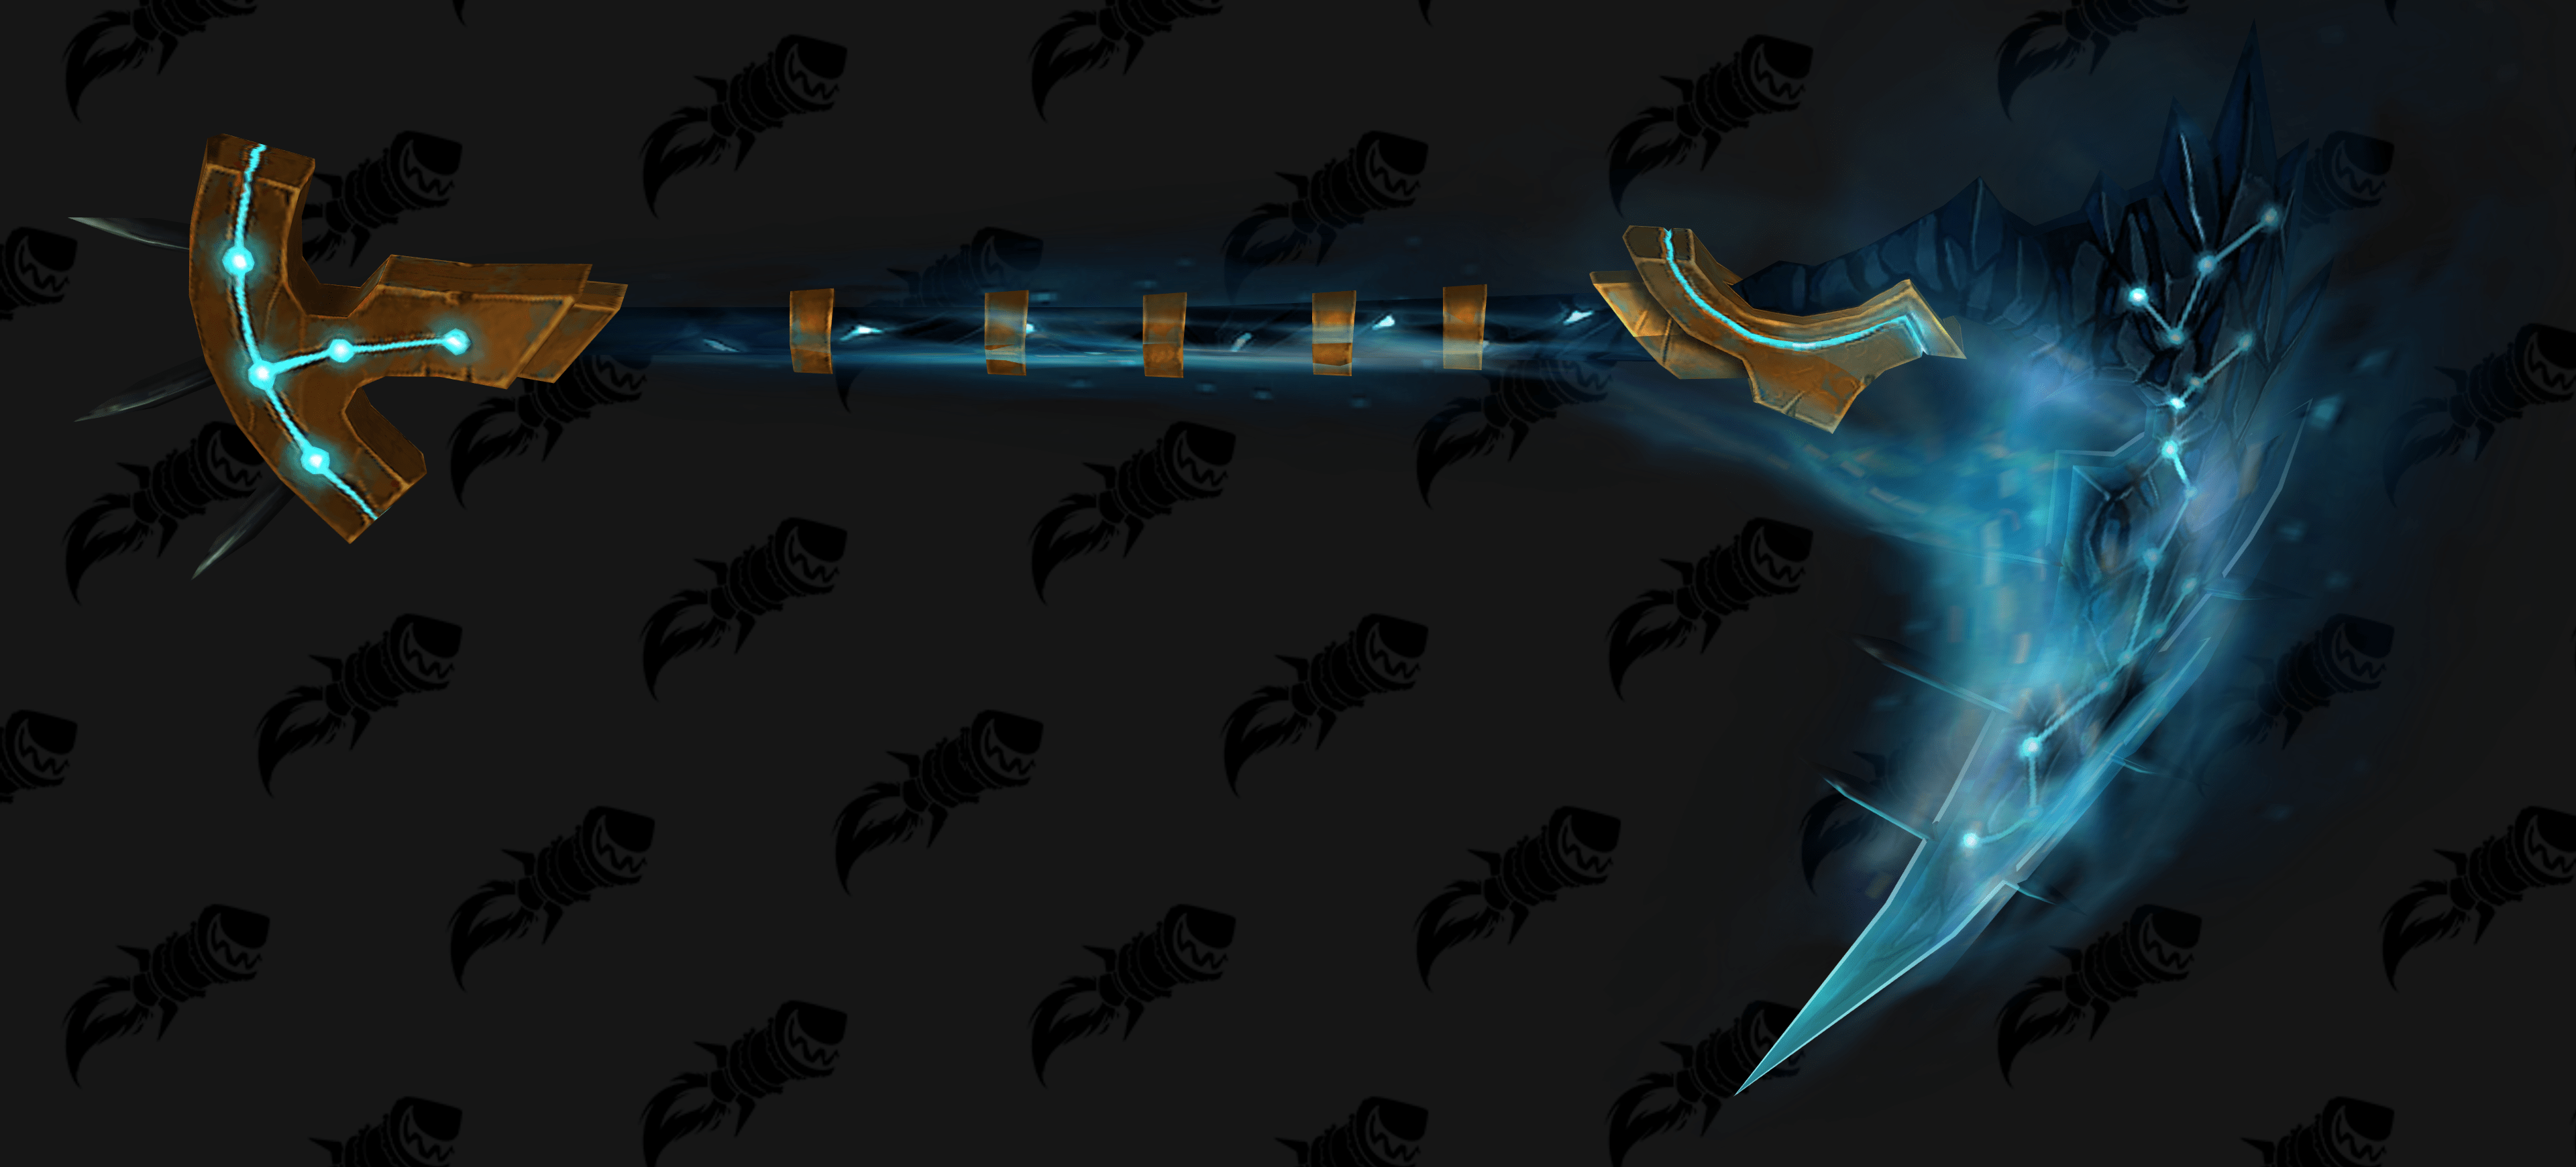
\includegraphics[width=\linewidth]{img/weapons/1213012.png}
\end{center}

\subsubsection{Potential}

The Scythe of the Unmaker seeks the souls of victims. It can try to influence the wielder to want to attack a target if it so desires the soul of them.

\begin{commentbox}{Scythe of the Unmaker\footnote{Weapon (scythe), artifact (requires attunement by a Grim Reaper)}}
	You gain a +3 bonus to attack and damage rolls made with this magic weapon. When you hit an enemy you will deal 2d4 psychic damage and 2d4 necrotic damage. The damage will change to d8's if the target has the opposite alignment of the wielder.
	
	The target of a melee attack of this scythe must make a constitution saving throw. On a fail, they take 5d6 psychic damage. The DC for this save is the wielders level + their constitution modifier.
	
	When the wielder rolls a 20 against a creature with the opposite alignment of the wielder, the wielder must a d100 roll. If the roll is less than half the wielders level then the creature will have its soul consumed within the scythe and become lifeless immediately.
	
	Any. When the wielder rolls a 20 against a character with good alignment the wielder must a d100 roll. If the roll is less than half the wielders level then the creature will have it's soul removed and become lifeless immediately.
	
	If a Grim Reaper of an good alignment tries to attune to The scythe they have to make a d20 roll. 
	\begin{enumerate}
		\item Chaotic good: At a 14 or below The scythe will reject you and deal 3d10 necrotic damage and 2d10 psychic damage. At a 14 or above you over power the will of the weapon and make it yours.
		\item Neutral good: At a 16 or below The scythe will reject you and deal 3d10 necrotic damage and 2d10 psychic damage. At a 16 or above you over power the will of the weapon and make it yours.
		\item Lawful good: At a 18 or below The scythe will reject you and deal 3d10 necrotic damage and 2d10 psychic damage. At a 19 or 20 you over power the will of the weapon and make it yours.
	\end{enumerate}
	
	Proficiency with a scythe allows you to add your proficiency bonus to the attack roll for any attack you make with it.
\end{commentbox}

\subsubsection{Finding the Scythe of the Unmaker}

The Scythe of the Unmaker is located in an ancient and haunted graveyard deep in the Pluvian Forest. The graveyard is centuries old and buried within an underground bog in the caverns of a large mountain. The scythe is help in the grave with an undead warlock necromancer. This necromancer found the scythe and tried to harness its power but utterly failed. After studying the scythe the necromancer tried to tap into its potential to resurrect fallen spirits from this graveyard, but instead was consumed in the process. In his death, the necromancer became entrapped by the power of the scythe becoming eternally dammed to be a keeper of the graveyard and protector of the scythe. When entering the graveyard, a horde of undead will awaken and attack anyone who dares intrude on the graves. The fallen necromancer will command them in protecting the scythe. If the necromancer is killed, the undead he commands will also fall.

\begin{monsterbox}{Necromancer}
	\begin{hangingpar}
		\textit{Medium Undead, lawful evil}
	\end{hangingpar}
	\dndline%
	\basics[%
	armorclass = 16,
	hitpoints  = 82,
	speed      = 30 ft
	]
	\dndline%
	\stats[
	STR = \stat{9}, % This stat command will autocomplete the modifier for you
	DEX = \stat{12},
	CON = \stat{14},
	INT = \stat{16},
	WIS = \stat{22},
	CHA = \stat{10}
	]
	\dndline%
	\details[%
	% If you want to use commas in these sections, enclose the
	% description in braces.
	% I'm so sorry.
	languages = {Common, undead},
	challenge = 6
	]
	\dndline%
	damage resistance = Necrotic, Poison
	
	condition immunities = Exhaustion, Petrified, Poisoned, Paralyzed, Feared	
	
	Senses = Passive Perception 20
	
	\dndline%
	\begin{monsteraction}[Horrify]
		All creatures within 60 ft. of you must make a DC18 constitution save. On a fail, they become frightened. On a success nothing happens and they become immune to your frightening glare for 24 hours.
	\end{monsteraction}	
	\begin{monsteraction}[Multiattack]
		You can take two attack actions per turn.
	\end{monsteraction}
	\monstersection{Actions}
	\begin{monsteraction}[Life Tap]
		As an action, you can make a melee spell attack against a living creature, dealing necrotic damage equal to 2d8 + your Charisma modifier on a hit. You gain temporary hit points equal to the amount of necrotic damage dealt. If this feature kills the creature, you gain twice as many temporary hit points from using this feature.
	\end{monsteraction}	
	\begin{monsteraction}[Melee Attack]
		Melee scythe attack. +5 to hit.
	\end{monsteraction}	
	\begin{monsteraction}[Confuse Soul]
		You blacken the mind of a living target. The target must make a DC16 wisdom save or lose a turn as their soul is struggling to stay connected to their physical bodies.
	\end{monsteraction}		
\end{monsterbox}


\begin{monsterbox}{Soulless Zombie}
	This character design is adapted from https://roll20.net/compendium/dnd5e/Zombie\#content
	\begin{hangingpar}
		\textit{medium undead, neutral evil}
	\end{hangingpar}
	\dndline%
	\basics[%
	armorclass = 8,
	hitpoints  = 22,
	speed      = 20 ft
	]
	\dndline%
	\stats[
	STR = \stat{13}, % This stat command will autocomplete the modifier for you
	DEX = \stat{6},
	CON = \stat{16},
	INT = \stat{3},
	WIS = \stat{6},
	CHA = \stat{5}
	]
	\dndline%
	\details[%
	% If you want to use commas in these sections, enclose the
	% description in braces.
	% I'm so sorry.
	languages = {All, cannot speak},
	challenge = 1/4
	]
	\dndline%
	saving throws = Wisdom +0
	
	damage immunities = Poison
	
	condition immunities = Poisoned	
	
	Senses = Darkvision 60 ft., passive Perception 8
	\dndline%
	\begin{monsteraction}[Undead Fortitude]
		If damage reduces the zombie to 0 hit points, it must make a Constitution saving throw with a DC of 5+the damage taken, unless the damage is radiant or from a critical hit. On a success, the zombie drops to 1 hit point instead.
	\end{monsteraction}	
	\monstersection{Actions}
	\begin{monsteraction}[Slam]
		Melee Weapon Attack: +3 to hit, reach 5 ft., one target. Hit: (1d4 + 1) bludgeoning damage. 
	\end{monsteraction}		
\end{monsterbox}

\section{Cleric Class Weapons}

\subsubsection{Chalice of Light}

The Chalice of Light is known in Legend to be a holy war hammer imbued directly with the presence of a divine spirit. It is believed that Apollo had a follower so loyal and faithful that Apollo sent an angel to reside within this particular war hammer and protect the wielder during his dangerous missionary journeys. The hammer was originally forged by a dwarven clan which dedicated themselves to Apollo. Per legend, a high priest of Apollo took it upon himself to set forth into the most dangerous lands to preach that of Apollo. Among his second journey, he found himself being ambushed and sent to his death in a place called The Undercity. In a fervent prayer, his war hammer became light to the tough, and changed it's appearance to hold an everlasting flame that burned alongside his faith and gave the high priest the ability to break free from his bonds and purge The Undercity of the sins that corrupted it and the surrounding lands. The flame of the burning hammer is said to have ceased when the wielder died of old age. It is believed that if the hammer is found, it is already forged to hold the essence of an angel and can provide uncanny abilities to a man of great faith.

\begin{center}
	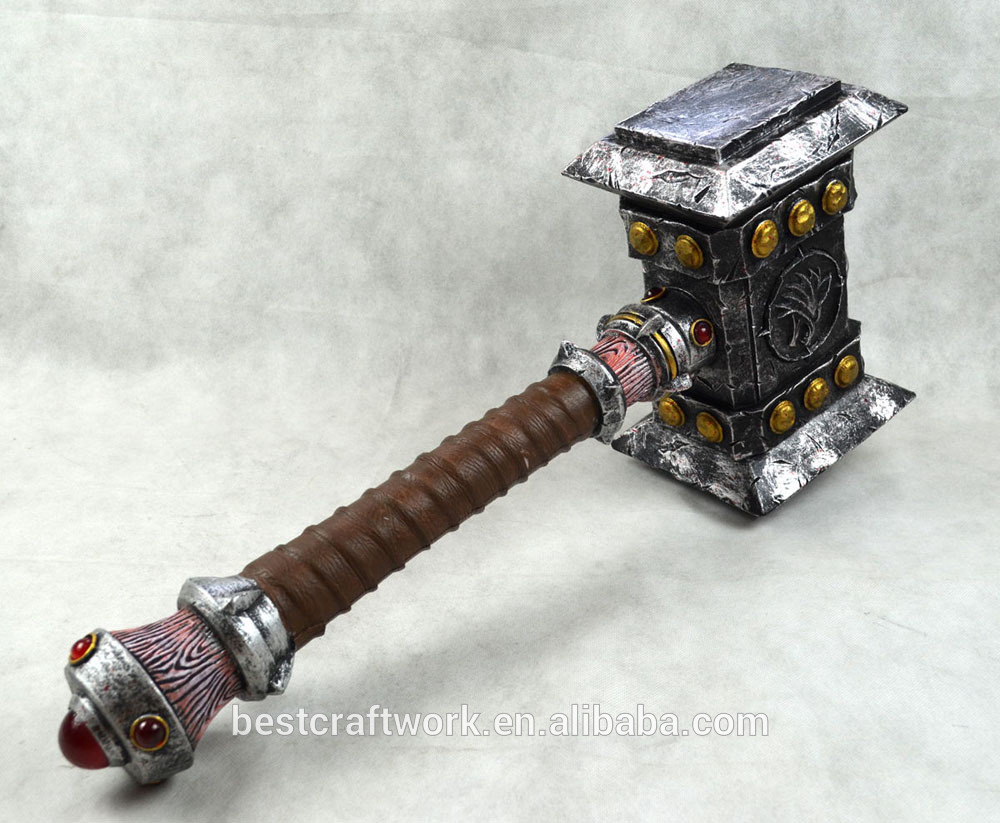
\includegraphics[width=0.41\linewidth]{img/weapons/Wow-Hammer.jpg} 	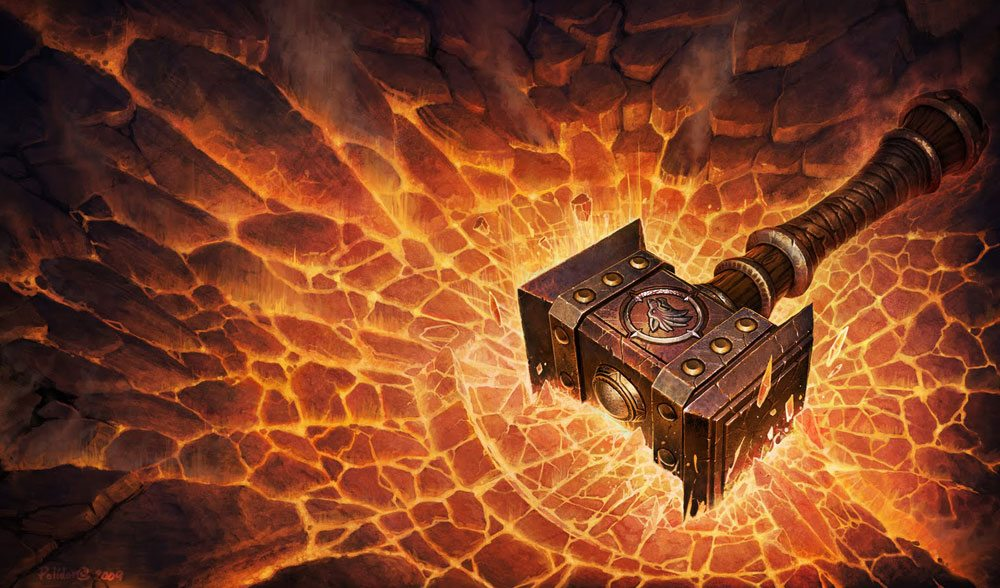
\includegraphics[width=0.57\linewidth]{img/weapons/shatteredhand.jpg}
\end{center}

\subsubsection{Potential}

The Chalice of Light weapon wants to be wielded by a religious character. 

\begin{commentbox}{Chalice of Light\footnote{Weapon (war hammer), artifact (requires attunement by a cleric)}}	
	If no angel or spirit from a deity is with this weapon, it is a simple warhammer that only does 1d8 bludgeoning damage.
	
	You gain a +3 bonus to attack and damage rolls made with this magic weapon. When you hit an enemy you will deal 1d6 fire damage and 1d6 radiant damage. The damage will change to d10's if the target rejects the clerics deity (they must know of them though).
	
	When you take damage while wielding the Chalice of Light, you can heal one target within 50 yards for a single roll of the dice closes to the wielders level (round up).
	
	While a cleric wields The Chalice of Light in combat it will look like the cleric is burning with a holy flame. Anyone who rejects the clerics deity that attacks the wielder will take 1d6 fire damage and 1d6 radiant damage. When the wielder rolls a 20 against someone who rejects their deity, a wielder must a d100 roll. If the roll is less than half the wielders lvl then the attacker will burn in holy flame and turn to ash immediately.
	
	If a cleric of an evil alignment tries to attune to The Chalice of Light they have to make a d20 roll. At a 18 or below The Chalice of Light will reject you and deal 3d10 fire damage and 2d10 radiant damage. At a 19 or 20 you over power the will of the weapon and make it yours.
	
	With a successful roll to overcome the will of The Chalice of Light while having an evil alignment will make The Chalice of Light's appearance will start to dull and become darker until it becomes fully corrupt. It will regain its former glory when its attuned to a cleric of a non evil alignment.
	
	Proficiency with a war hammer allows you to add your proficiency bonus to the attack roll for any attack you make with it.
	
	If the wielder of Chalice of Light dies (by failing three death saves) then the angel within the hammer can leave the weapon and resurrect the player to full. The weapon after this point becomes useless.
\end{commentbox}


\subsubsection{Finding the Chalice of Light}



\section{Fighter Class Weapons}

\subsubsection{}

\subsubsection{Potential}

\subsubsection{Finding }

\section{Other Artifact Weapons}

\subsection{Frostmourne}



\subsubsection{Potential}

Frostmourne is a cursed blade which can either torment the soul of the wielder or provide them with immense power.

\begin{commentbox}{Frostmourne}
	
\end{commentbox}

\subsubsection{Finding Frostmourne}